
We have implemented end-user programming approach and evaluated it to explore the following research questions:

(RQ1) What is the accuracy of the instruction recognize approach and how to improve the accuracy of it? (Chapter 5.1)

(RQ2)To what extent can user programming complexity be reduced by using this end-user programming approach? (Chapter 5.2)

(RQ3)Does our approach have an impact on efficiency in end-user programming? (Chapter 5.3)

\subsection{Accuracy of Program Instruction Conversion}

\subsubsection{Experimental Setup}

\paragraph{}
To evaluate the accuracy of our program instruction conversion method, we use 3 data sets: a Base set, a Paraphrase set and a Scenario set. All together, 2304 sentences are collected, of which 1424 are primitive and 680 are compound.

The instructions in the Base set are generated by the generation rules in Section 4.2. The Base set provides the basic instructions for the Smart Home Service, which enables basic control of various devices and functions. A total of 200 instructions are generated in our Base set which consists of 121 primitive sentences and 79 compound sentences.

The instructions in the Paraphrase set are written by trained labor who are familiar with the devices and functions in this smart home scenarios. The Paraphrase set is used to increase the variety of instructions in order to simulate the user's use of smart home devices in real-world scenarios as much as possible. 1057 sentences are collected, of which 714 are primitive and 343 are compound.

The instructions in the Scenario set are given by the volunteers. They are not familiar with the various devices and functions in this smart home scenarios. And the way they know about the devices and functions in this smart home only through our simple oral description and demonstration. Then volunteers give control instructions which based on their experience and understanding of smart home scenarios. We collected more natural sentences by using this approach. The Scenario set has 1047 instructions, including 710 primitive instructions and 337 compound instructions.

We compare the approach of this paper with the rule based approach [1] and the Almond approach [2] in the accuracy of instructions conversion. The rule based approach establishes series of instructions recognition rules and determines the sentence pattern according to the syntax structure for each instruction. It uses the syntax dependency relationship to find information such as actions, device names, place names and context attributes in the instructions. Finally, according to the defined knowledge inference rules, it matches the device, location, and context in the runtime knowledge graph, thereby mapping the instruction to a specific service that can implement the function.The Almond approach obtains information through Thingpedia entries and use machine learning to train the Thingtalk program and its paraphrase to obtain a semantic parser. Finally, the semantic parser is used to parse the user's instructions to match programs. There is only one result for the rule based approach. We measure if the correct answer is among the top 1, 3, and 5 matches in both our approach and the Almond approach


\subsubsection{Analysis of Results}
\paragraph{}

\begin{figure}[h]
\centering
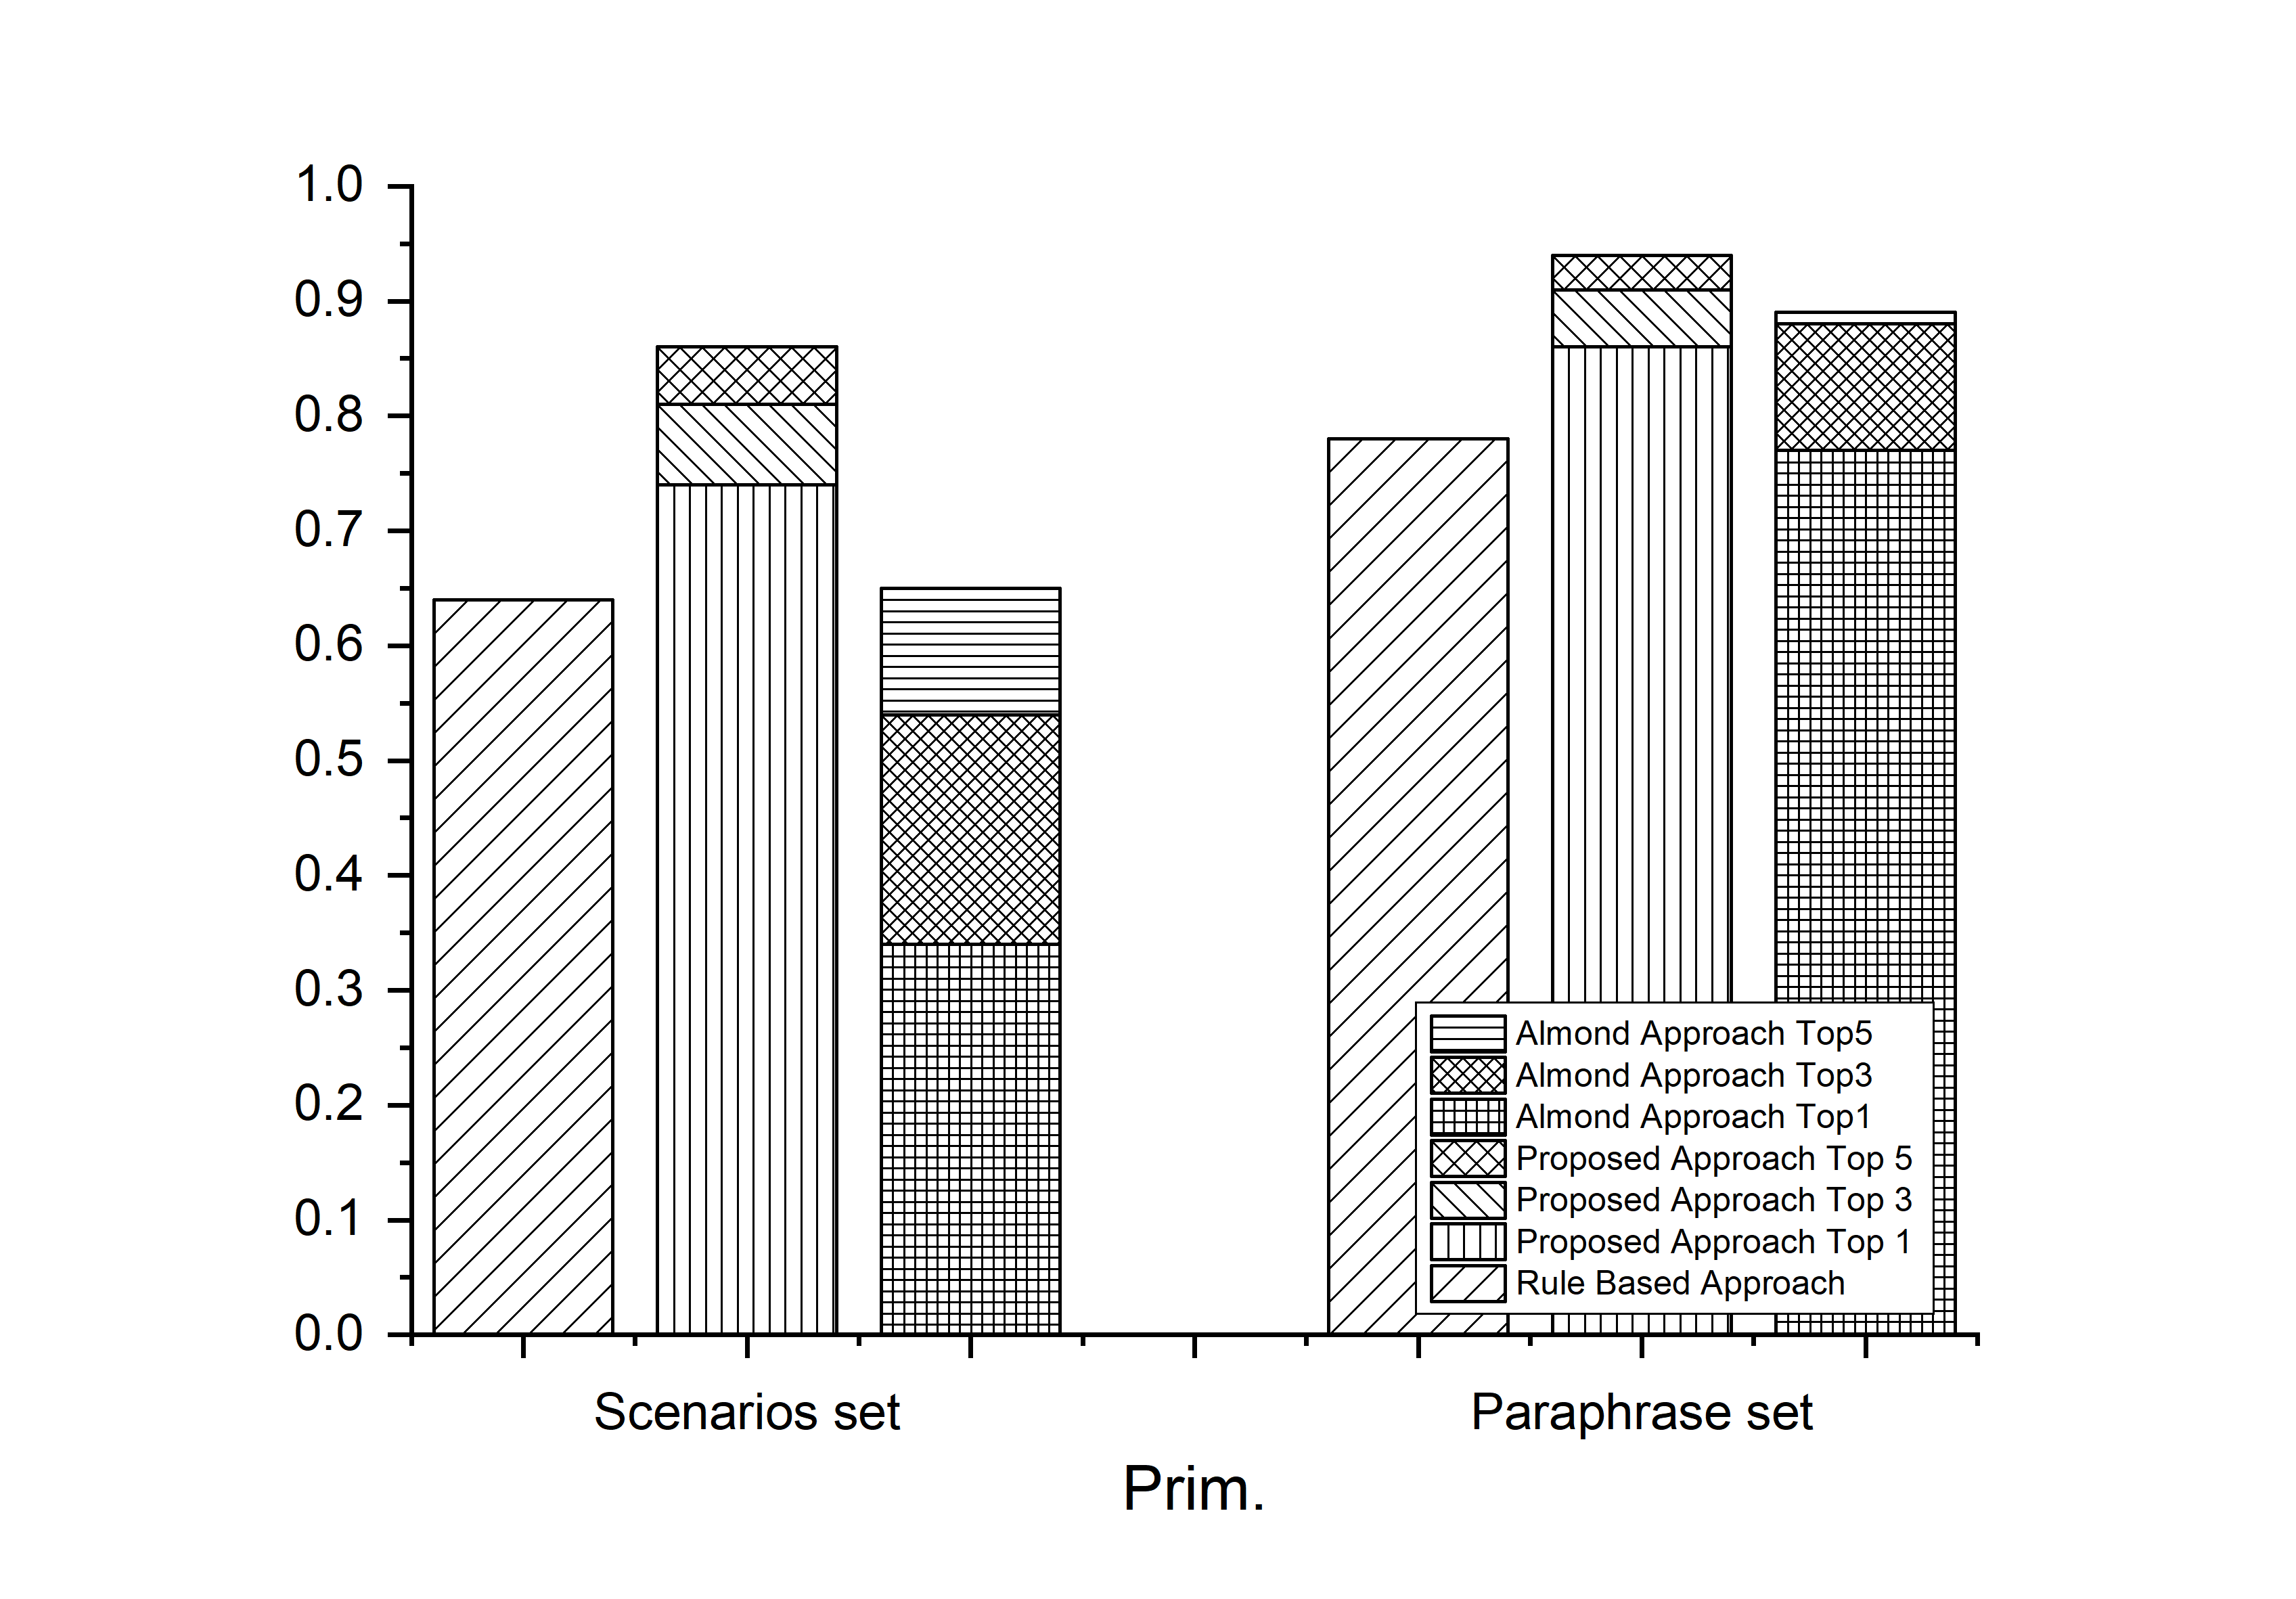
\includegraphics[width = .5\textwidth]{fig5_1.png}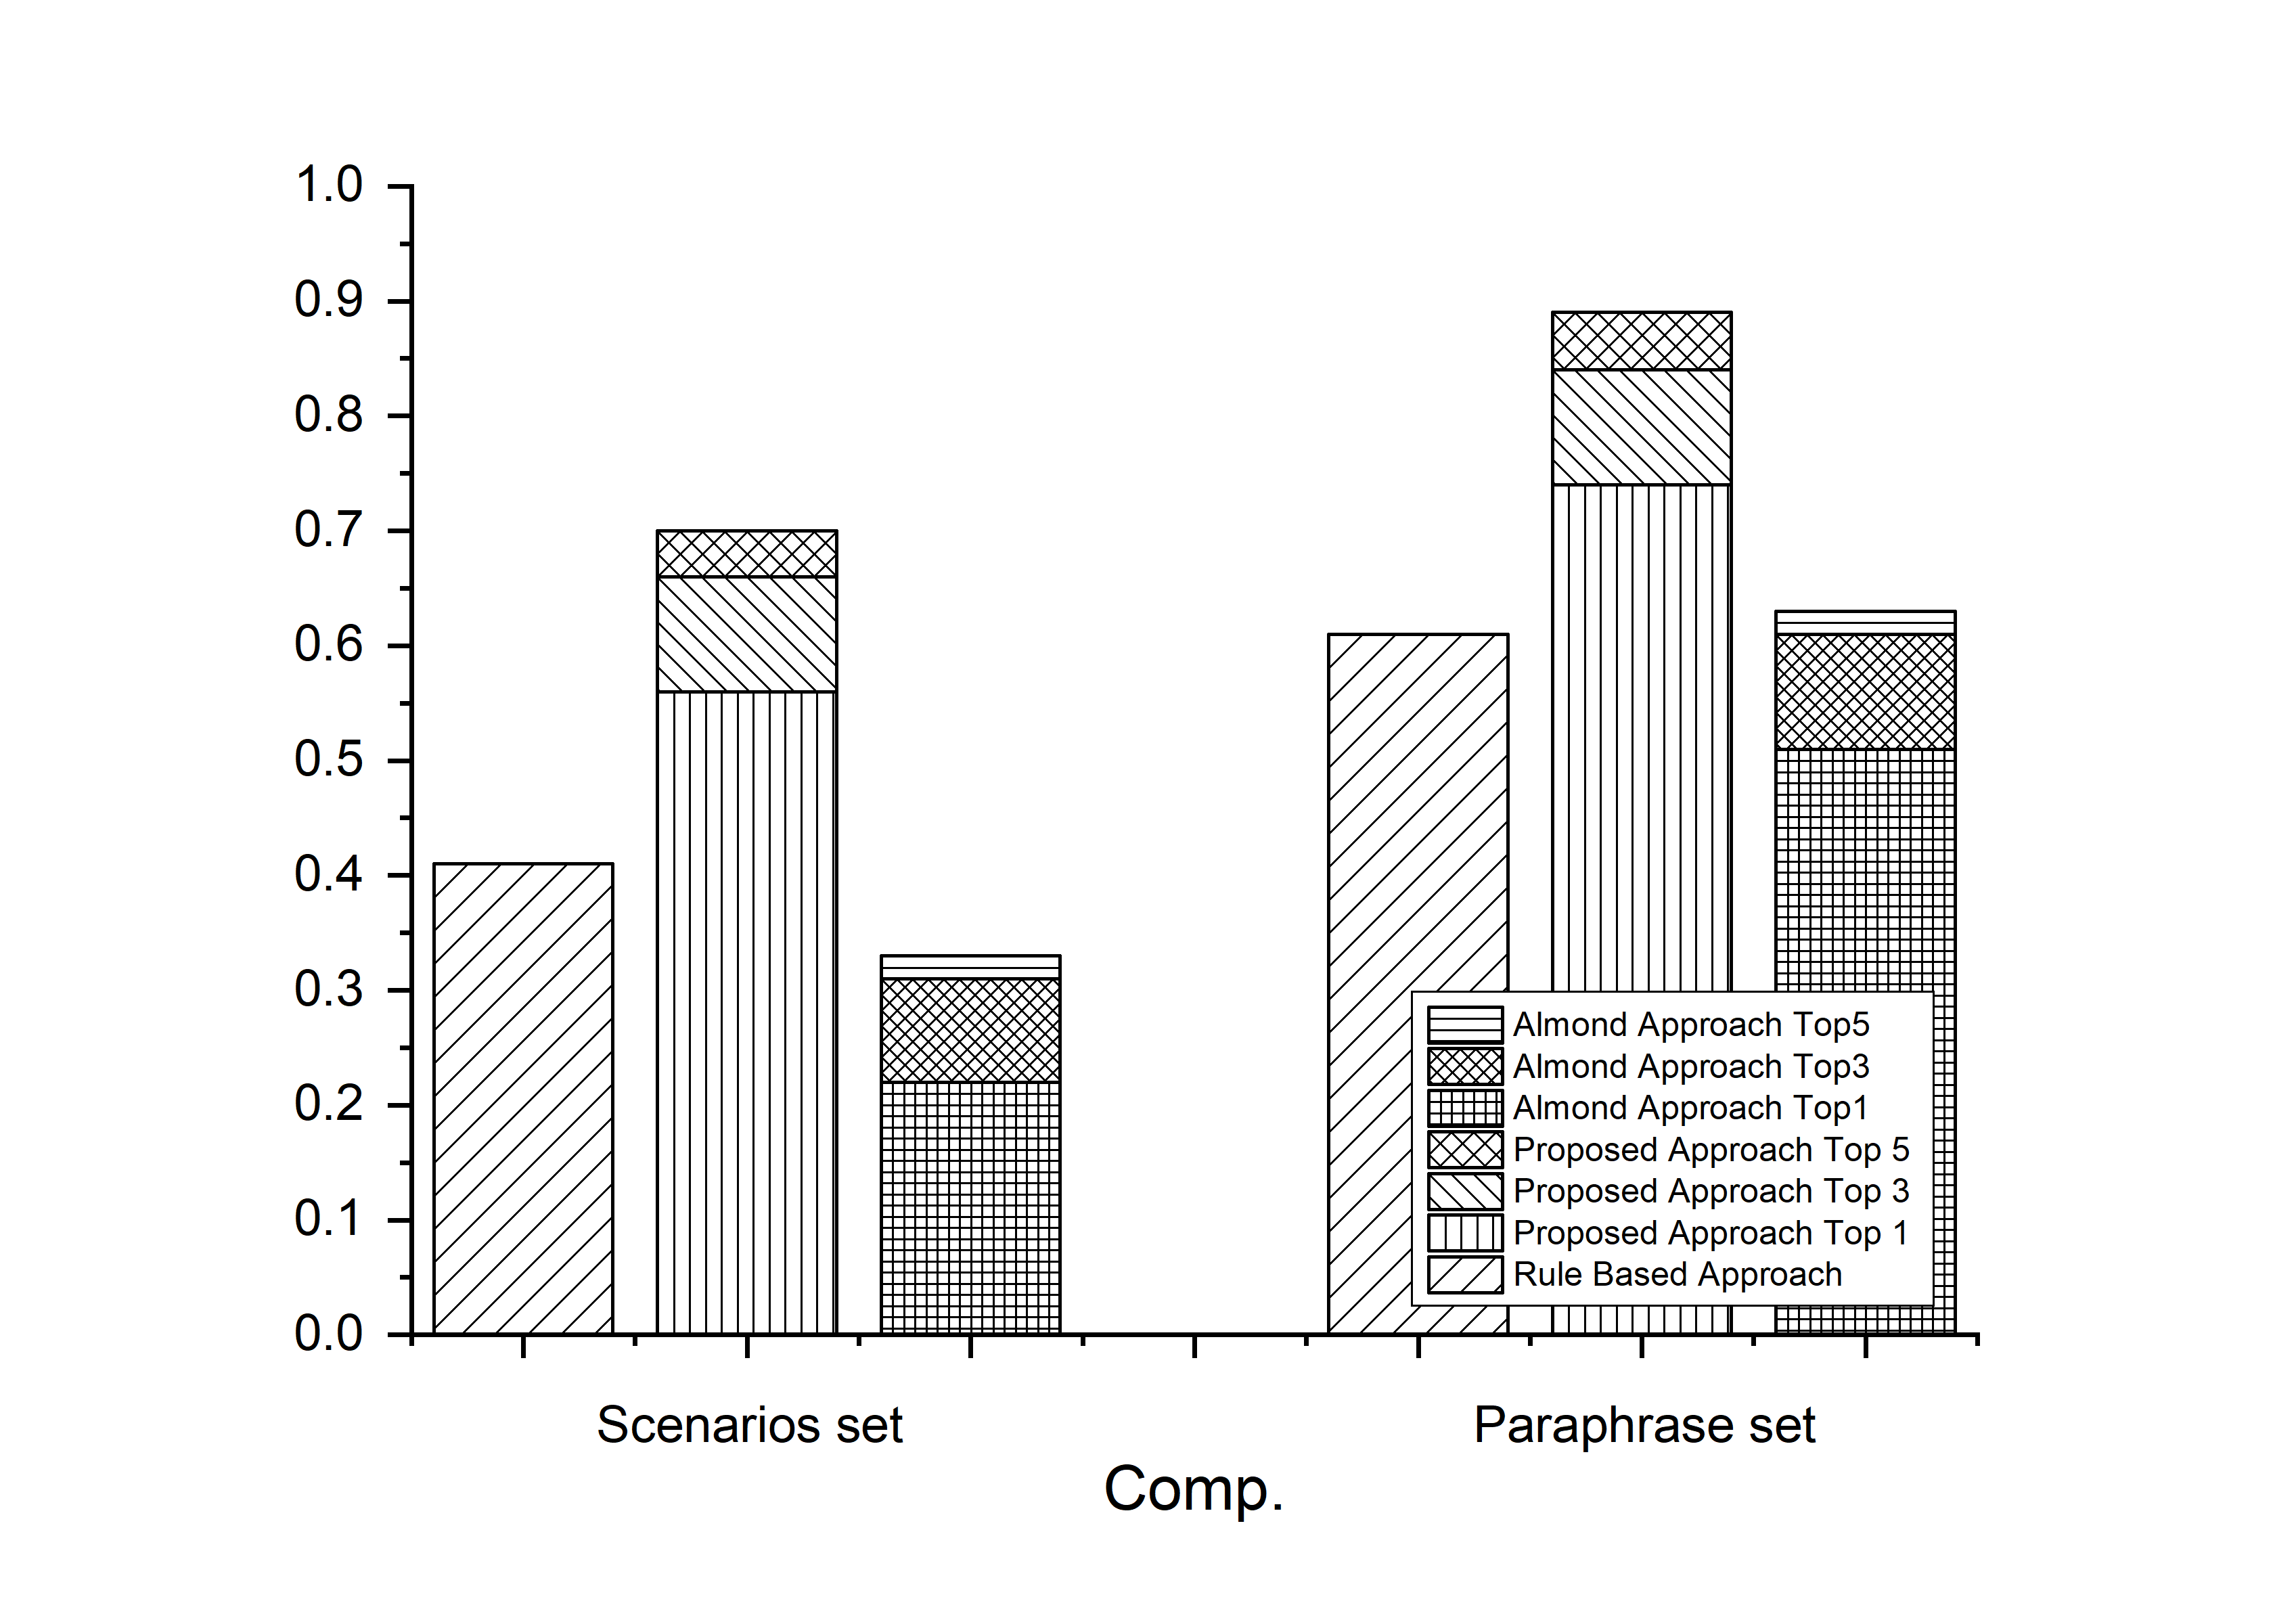
\includegraphics[width = .5\textwidth]{fig5_2.png}
\caption{Instructions Recognition Accuracy of Three Approaches}
\end{figure}
The experimental results are shown in Fig.5.The left shows the accuracy of recognition of the primitive instructions by rule based approach, our approach and Almond approach in the three sets. The right shows the accuracy of recognition of the compound instructions by rule based approach, our approach and Almond approach in the three sets.

In the Base set, the accuracy of the rule based approach, our approach and Almond approach are all 100\%. This is because the Base set is composed of instructions which are generated by the rules defined in Section 4.2. Therefore these approaches can accurately recognize these most basic instructions.

In the Paraphrase set, you can see that the accuracy of the rule based approach on the primitive instructions is 77\%. Because the rule based approach can only recognize the sentence structure and specification defined by rules in the text. Once the sentence structure or lexical representation becomes undefined ,the approach cannot recognize the instructions any more. The accuracy of the rule based approach in the recognition of compound sentences is only 61\%. Because the structure of compound instructions are too complex and diverse. If you need to recognize them accurately, you have to define a large number of rules for each type of sentence. It cannot be defined one by one obviously. For example, if the marker words of the condition in the compound sentence are not defined, the sentence structure will change and it will not be recognized. In our approach, the Top1 recognition accuracy of the primitive instructions is 86\%, Top3 is 91\%, and Top5 is 94\%. Our approach can solve the problem of sentence structure and partial word change. However, because of the limitations of the natural language processing method used in this paper, it still causes some groups of synonym to be unrecognizable, such as device operation "turn down" should be recognized as "reduce". However, it will match the "turn off" with higher similarity of the word vector in practice . Our approach obtained an accuracy of 74\% at Top 1 in the compound instructions, 84\% at Top3, and 89\% at Top5. Its recognition accuracy is about 5\%~12\% lower than primitive instructions. Because we split the compound instruction into two primitive instructions and matches separately. Then we synthesize the compound instructions according to the compound instructions combination strategy of 4.3 and it will display five matching results. In the matching of compound instructions, only the two primitive sentences that make up it match correctly, which can be correctly recognized. Therefore, it will make the accuracy to drop . In the Almond approach, the Top1 recognition accuracy of the primitive instructions is 77\%, Top3 is 88\%, Top5 is 89\%, the compound instructions Top1 recognition accuracy is 51\%, Top3 is 61\%, Top5 is 63\%. On the one hand, the Thingpedia of Almond is an open domain-based knowledge base. If you want to improve the accuracy of instructions in a specific field, you have to train in advance for that particular field, which requires extra work. On the other hand, because of the training of the Almond is not oriented to the smart home scenario, so the accuracy of the operation instructions directly to the device in this scenario is not as good as our approach.

In the Scenario set, There are more complex and colloquial instructions than Paraphrase set. It greatly increase the challenge of instruction recognition. The Scenario set contains many highly abstract instructions that make our approach and the other two approaches can not recognize the instruction. In primitive instructions, the accuracy of the rule based approach is 64\%. Our approach obtains an accuracy of 74\% in Top1, 81\% in Top3, 86\% in Top5. Almond approach obtained an accuracy of 34\% in Top1, 54\% in Top3 and 65\% in Top5.In compound Instructions, the accuracy of the rule based approach is 41\%, our approach obtains an accuracy of 56\% in Top1, 66\% in Top3, 70\% in Top5. Almond approach obtained an accuracy of 22\% in Top1, 31\% in Top3, 33\% in Top5. The reason for the low accuracy is mainly due to the volunteers' various semantic and complex instructions which based on their life experience and the given smart home scenario. For example, volunteers may give an abstract condition such as "if the sitting room is well lighted" when setting the room brightness service. At this time, the rule based approach, our approach and the Almond approach will not understand the semantics and recognize wrongly. However, our approach instruction recognition rate is higher than the other two approaches, because we define a series of “Context” entities on the knowledge graph which is based on the smart home scenario. So our approach can recognize some of the instructions with high-level semantics and then the instruction recognition accuracy is lower than the other two approaches. For example, for the living room air quality query "How is the air quality of the living room?", the rule based approach and the Almond approach cannot understand the specific meaning of "air quality", and our approach defines the “Context” of the concentration of PM2.5 in the living room. So we can know that this query instruction is asking about the air quality in the living room, and finally correctly matches the instruction "What is the PM2.5 in the sitting room ?". Then it will execute Get $C_i.CValue$ to get the concentration of PM2.5 in the living room air. 

In primitive instructions, the accuracy of the rule based approach is reduced by 14\% compared to the Paraphrase set. The accuracy of our approach is reduced by 8\% to 12\%, and the accuracy of the Almond approach is reduced by 24\% to 43\%; In compound instructions, the accuracy of the rule based approach is reduced by 23\% compared to the Paraphrase set, the accuracy of our approach is reduced by 18\% to 19\%, and the accuracy of the Almond approach is reduced by 29\% to 30\%.

This shows that in our “Context” entity which defined in the knowledge graph with scenario, it can really improve the recognition accuracy of some high-level semantic instructions in the smart home scenario.

In summary, our approach can not only recognizes instructions generated by rules, but also has a high recognition accuracy for instruction sets written by trained testers. It can also adapt to scenes to understand some more semantically complex instructions.

\subsection{Reduction for Lines of Code}

Table 12 displays the comparison of LOC between the two approaches for smart home situational awareness services . When using Java to develop these services, each service is developed independently. While using the approach of this paper, developers only need to implement scenario-oriented configuration, that is, the base code which has 115 lines. In the development for these service by Java, the codes of interface calls are the codes of underlying device interface calls. The approach of this paper only requires users to give instructions. Then the parser will parse through the underlying code. And we use the runtime knowledge graph to achieve the same function without adding any redundant code. For example, $S_{11}$ is Jack's temperature adjustment service, and the lines of code for the Java program are 220, where the codes of interface calls are 136 lines, the management logic codes are 84 lines. $S_{23}$ is Ken's air conditioning service, the Java program has 140 lines of code, wherein the interface call codes are 68 lines, management logic codes are 72 lines. The average lines of code for a Java program are 186 lines, and the average lines of code for the approach of this paper only require 10 lines. So the code reduction is over 94.8\%.

\begin{table}[h]
	\centering
	\begin{tabular}[h]{|c|c|c|c|c|c|c|c|c|c|c|c|c|c|c|c|}				
		\hline
		& Basic& $S_{11}$ & $S_{12}$ & $S_{13}$ & $S_{21}$ & $S_{22}$ & $S_{23}$ & $S_{31}$ & $S_{32}$& $S_{41}$ & $S_{42}$& $S_{51}$ & $S_{52}$&Average\\
		\hline
		Java & 0 & 220 & 198  & 140 & 220 & 198  & 140 & 220& 197  & 163 & 188& 163  & 188 & 220\\
		\hline
		Our Approach & 115 & 0 & 0 & 0 & 0 & 0& 0 & 0 & 0& 0 & 0 & 0 &0&10\\
		\hline		
	\end{tabular}
	\caption{Comparison in LOC of Two Approaches}	
\end{table}

\subsection{Program Execution Time}

\begin{figure}[h]
	\centering
	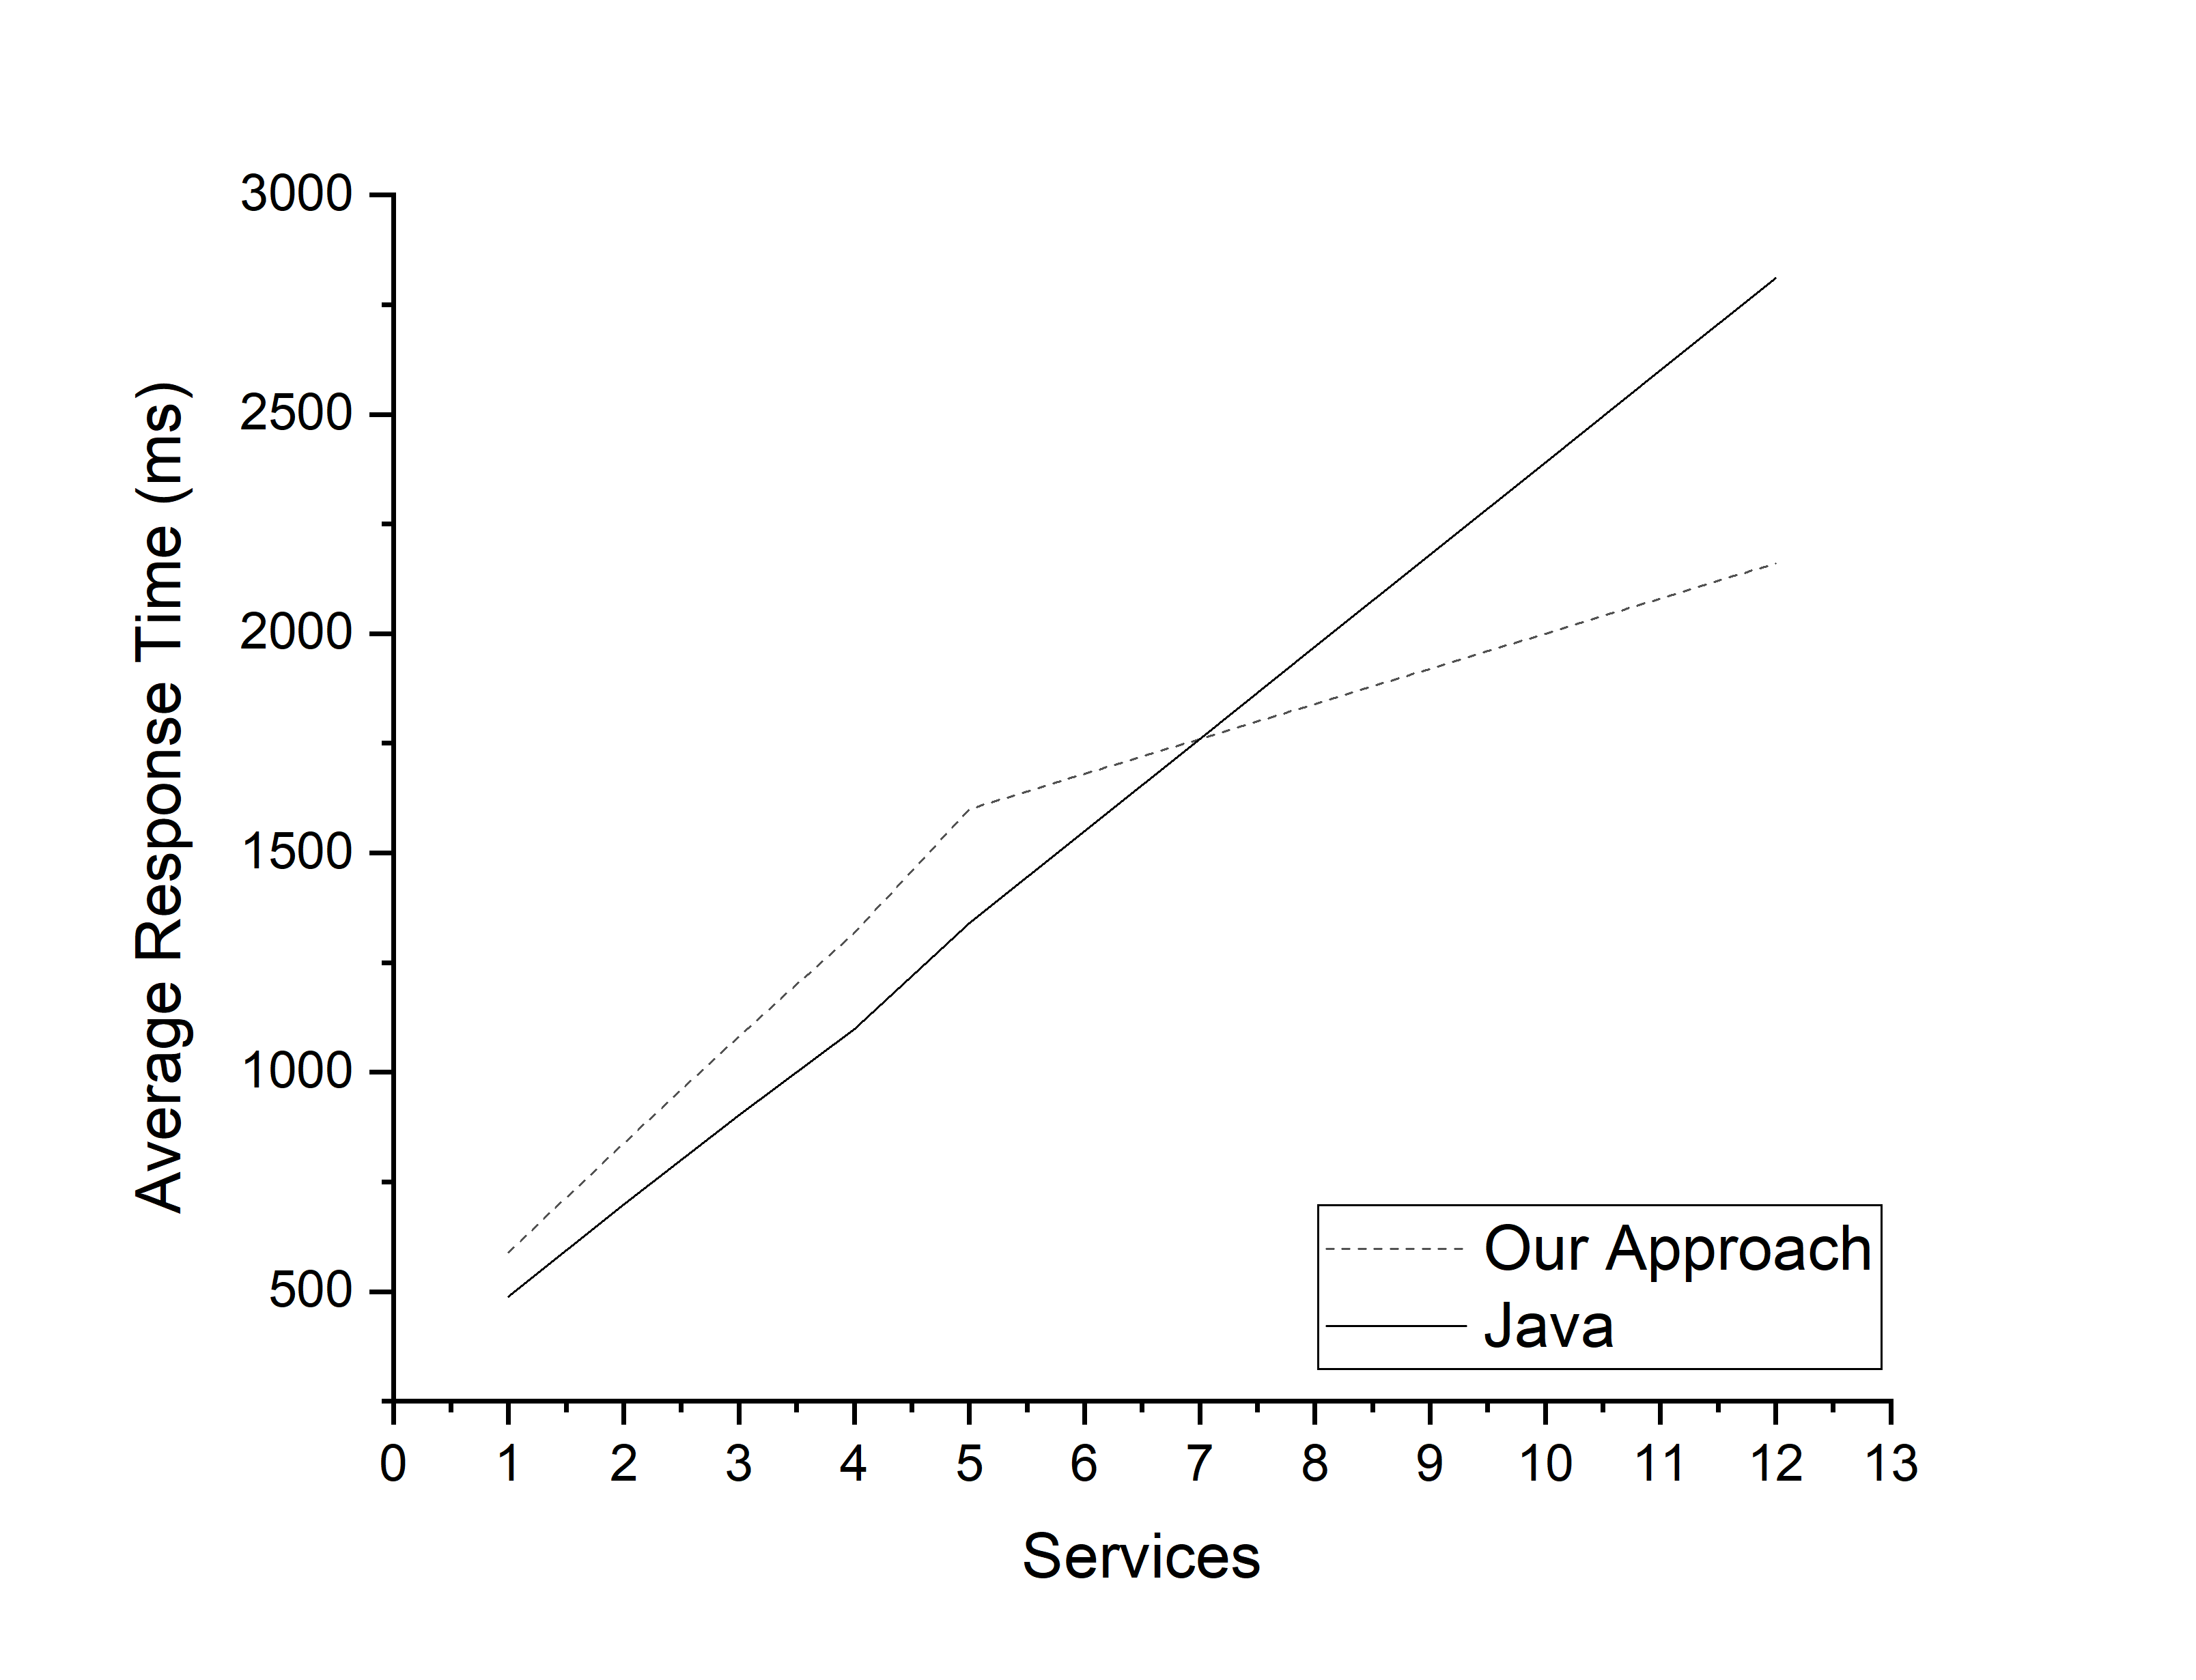
\includegraphics[width = .8\textwidth]{fig6.png}
	\caption{Comparison in Execution Time of Two Approaches}
\end{figure}

In order to compare the service execution performance between the two approaches. The development environment is a server with 3.1GHz 4Core CPU, 4GB RAM. Different numbers of smart home situational awareness services are executed. The average response time is counted,which is shown in Figure 6. In a Java program, each service is executed sequentially. The management logic is executed separately and the device APIs are called. Therefore, the average response time increases linearly with the number of services. When using the approach of this paper, the knowledge graph instance model is transformed by the model operation and the device API calls to realize two-way synchronization with real-time information of the scenario. On this basis, knowledge reasoning is performed according to service requirements. On the one hand, additional operations are needed to maintain the runtime synchronization of the instance model and the smart home scenarios. When the number of services is small, the average response time of this approach is higher than Java programs. For the perspective of intelligent services, this difference in performance is acceptable. On the other hand, the services in the Java program are executed independently, when the service reaches a certain number, so there will be cases that different context aware services call the same device API to obtain scene information (for example, $C_{11}$, $C_{21}$ and $C_{31}$ are all to monitor the living room temperature). When there is a large number of services,the proposed approach can effectively reduce the overhead equipment API called repeatedly generated so that the average response time is low.


